\documentclass[12pt,a4paper]{article}

% ── Packages ───────────────────────────────────────────────────────────────────
\usepackage[utf8]{inputenc}
\usepackage[T1]{fontenc}
\usepackage[english]{babel}
\usepackage{amsmath,amssymb,amsfonts}
\usepackage{graphicx}
\usepackage{hyperref}
\usepackage{listings}
\usepackage{booktabs}
\usepackage{array}
\usepackage{xcolor}
\usepackage{geometry}
\usepackage{cite}
\usepackage{algorithm}
\usepackage{algpseudocode}
\usepackage{tikz}
\usetikzlibrary{shapes.geometric, arrows, positioning}

\geometry{margin=1in}

\hypersetup{
  colorlinks=true,
  linkcolor=blue,
  citecolor=blue,
  urlcolor=blue
}

\lstset{
  basicstyle=\small\ttfamily,
  breaklines=true,
  frame=single,
  backgroundcolor=\color{gray!10}
}

% ── Title ──────────────────────────────────────────────────────────────────────
\title{\textbf{LICET: A Cryptographic Protocol for Multi-Modal Physiological\\
Human-Intent Verification in Autonomous AI Agent Authorization}}

\author{
  Christian Rodrigues Pereira\\
  \textit{eColabs Desenvolvimento de Pessoas e Organizações LTDA.}\\
  CNPJ 43.694.779/0001-03\\
  \href{mailto:contato@ecolabs.com.br}{contato@ecolabs.com.br}\\
  \href{https://licet.dev}{https://licet.dev}
}

\date{July 2026 — v2.0\\[0.5em]
\small Preprint — SSRN Abstract ID: 7018458 · IETF draft-pereira-licet-human-intent-01}

% ══════════════════════════════════════════════════════════════════════════════
\begin{document}
\maketitle

% ── Abstract ──────────────────────────────────────────────────────────────────
\begin{abstract}
As autonomous AI agents gain the capacity to execute consequential actions in
high-stakes domains—medical prescribing, financial transactions, critical
infrastructure control—existing authorization mechanisms fail to answer a
fundamental question: \textit{was the authorizing human genuinely conscious,
uncoerced, and cognitively capable at the exact moment of authorization?}
Passwords, static biometrics, and digital signatures verify \emph{identity},
not \emph{intent state}.

We present \textbf{LICET} (Latin: \textit{it is permitted}), a middleware
protocol that cryptographically binds AI agent authorization events to the
real-time physiological state of the authorizing human via a three-layer
architecture: (1) an \textbf{identity anchor} using ECG waveform morphology—an
anatomically determined signal resistant to pharmacological manipulation; (2) a
\textbf{liveness layer} using continuous electrodermal activity (EDA) and
overnight HRV pattern matching, proving the presence of a conscious biological
subject; and (3) a \textbf{voluntary state layer} using personalized Mahalanobis
distance fusion across five physiological channels with pharmacological attack
pattern detection.

LICET additionally provides: (iv) per-event session-key derivation via HKDF;
(v) a Schnorr zero-knowledge proof over BN128, enabling third-party audit without
exposing biometric data; (vi) a SHA-256 hash-chained ledger providing
tamper-evident authorization records; and (vii) a four-level biometric trust
hierarchy (L0--L3) aligned with IETF RATS architecture (RFC~9334), enabling
progressive hardware assurance as wearable attestation technology matures.

The protocol is designed as a \textbf{coercion cost elevation mechanism}: no
single pharmacological intervention—beta-blockers, anticholinergics, opioids, or
their combination at survivable doses—defeats the multi-signal fusion system. A
reference implementation is publicly deployed at
\href{https://licet.dev}{\texttt{licet.dev}}. LICET addresses EU AI Act
operational oversight obligations (Articles~9, 12, and 26) and Brazil's LGPD
biometric data provisions.
\end{abstract}

\textbf{Keywords:} AI safety, human oversight, zero-knowledge proofs,
biometric authentication, autonomous agents, physiological attestation,
electrodermal activity, ECG morphology, IETF RATS, coercion resistance

% ──────────────────────────────────────────────────────────────────────────────
\section{Introduction}
% ──────────────────────────────────────────────────────────────────────────────

Artificial intelligence agents are transitioning from passive tools to
autonomous actors capable of executing actions with real, irreversible
consequences. A medical AI agent may adjust insulin doses. A financial AI may
execute wire transfers. An infrastructure AI may modify power-grid parameters.
In each case, the assumed safeguard is human authorization—yet current
authorization mechanisms carry a structural flaw.

\subsection{The Intent Gap}

Contemporary authorization primitives—passwords, FIDO2 keys, fingerprint
readers, iris scanners—are designed to answer one question: \textit{is this
person who they claim to be?} They are silent on a second, equally critical
question: \textit{is this person currently in a state that constitutes
genuinely free, conscious, and cognitively competent intent?}

Table~\ref{tab:intent-gap} contrasts existing mechanisms against the
authorization properties required for high-stakes AI agent actions.

\begin{table}[h]
\centering
\caption{Authorization properties of existing mechanisms vs.\ LICET v2.}
\label{tab:intent-gap}
\begin{tabular}{lccccc}
\toprule
\textbf{Mechanism} & \textbf{Identity} & \textbf{Liveness} &
\textbf{Coercion-elevated cost} & \textbf{Cognitively intact} &
\textbf{Drug-resistant} \\
\midrule
Password          & $\sim$ & \texttimes & \texttimes & \texttimes & \texttimes \\
Static biometric  & \checkmark & \checkmark & \texttimes & \texttimes & \texttimes \\
FIDO2 / passkey   & \checkmark & \checkmark & \texttimes & \texttimes & \texttimes \\
Digital signature & \checkmark & \texttimes & \texttimes & \texttimes & \texttimes \\
HR/HRV threshold  & \texttimes & \checkmark & $\sim$ & $\sim$ & \texttimes \\
\textbf{LICET v2} & \checkmark & \checkmark & \checkmark & \checkmark & \checkmark \\
\bottomrule
\end{tabular}
\end{table}

\subsection{Motivating Scenarios}

\begin{enumerate}
  \item \textbf{Healthcare:} An AI agent requests authorization from a physician
  to administer a controlled substance. The physician is under physical duress.
  LICET's EDA layer detects acute sympathetic arousal inconsistent with voluntary
  state and refuses the authorization.

  \item \textbf{Finance:} An AI system requests approval for a large wire
  transfer. The authorizer has taken a beta-blocker to suppress HR and HRV
  responses, but LICET detects the pharmacological attack signature (tremor
  amplitude below personal baseline, HR-HRV dissociation) and flags the
  session as \texttt{SUPPRESSED}.

  \item \textbf{Critical infrastructure:} An autonomous operations agent
  requests permission to modify a power distribution substation. LICET's
  three-layer verification confirms identity via ECG morphology, liveness via
  EDA reactivity, and voluntary state via multivariate deviation analysis.

  \item \textbf{Legal:} An AI contract agent requires authorization to sign a
  binding agreement. LICET's ZKP provides cryptographic proof of physiological
  state at signing time without exposing any biometric values to the auditor.
\end{enumerate}

\subsection{Contributions}

This paper makes the following contributions:
\begin{itemize}
  \item A three-layer physiological authorization architecture (Identity +
  Liveness + Voluntary State) addressing the limitations of single-signal
  threshold approaches.
  \item Introduction of ECG waveform morphology as a medication-resistant
  biometric identity anchor for authorization systems.
  \item A personalized Mahalanobis distance fusion model replacing
  population-level thresholds, with pharmacological attack pattern detection.
  \item A four-level biometric trust hierarchy (L0--L3) aligned with IETF RATS
  architecture (RFC~9334) \cite{rfc9334}, enabling progressive hardware
  assurance as wearable attestation technology matures.
  \item A formal specification of the target Level~3 (sensor-to-TEE direct
  attestation) architecture that does not yet exist in consumer hardware,
  defining the standard future wearable implementations should meet.
  \item A zero-knowledge proof scheme (Schnorr/BN128) enabling auditable
  authorization without biometric data exposure.
  \item A hash-chained ledger design providing mathematically verifiable,
  tamper-evident authorization history.
  \item A working reference implementation, publicly accessible at
  \href{https://licet.dev}{\texttt{licet.dev}}.
\end{itemize}

% ──────────────────────────────────────────────────────────────────────────────
\section{Related Work}
% ──────────────────────────────────────────────────────────────────────────────

\subsection{Human Oversight in AI Systems}

The EU AI Act \cite{euaiact2024} mandates human oversight for high-risk AI
systems across multiple provisions. Article~9 requires a risk management
system including ongoing monitoring of authorized human oversight.
Article~12 mandates logging of events for post-hoc audit. Article~26(5)
imposes deployer obligations to ensure that human oversight is \emph{genuinely
exercised}---not merely that an authorization button was pressed. LICET
provides the technical substrate for these operational assurance obligations:
the physiological attestation layer creates a machine-verifiable record that
oversight was not bypassed under duress or incapacitation.

Note on Article~14: this provision concerns the AI system's design capacity
for human oversight---it specifies that systems must be designed to allow
humans to understand, monitor, and intervene. LICET addresses the
complementary operational question: whether the human exercising that capacity
was physiologically capable of doing so genuinely. These are distinct
requirements within the same regulatory framework.

NIST AI RMF \cite{nistairimf2023} introduces the concept of ``human in the
loop'' without defining a cryptographic binding between oversight events and
authorization records. LICET provides the missing technical substrate.

\subsection{Multi-Modal Physiological Stress Detection}

The WESAD dataset \cite{schmidt2018wesad} established the benchmark for
wearable multi-signal physiological stress detection, demonstrating that
EDA + HRV + skin temperature fusion achieves approximately 85--88\% three-class
accuracy (baseline/stress/amusement), substantially outperforming any single
signal. Healey and Picard \cite{healey2005stress} demonstrated multi-signal
fusion superiority in real-world conditions using EDA, HR, and skin
conductance. LICET extends this literature to the specific adversarial context
of coercion and pharmacological countermeasures, applying personalized
baselines rather than population models.

\subsection{Biometric-Based Coercion Detection}

Research on physiological stress markers dates to the foundational work of
Selye \cite{selye1956stress}. The autonomic nervous system's sympathetic
activation under acute stress produces measurable concurrent elevation of heart
rate and suppression of heart rate variability \cite{thayer2012hrv,
kim2018stress}. Prior work in duress-code systems \cite{Capkun2006} explored
covert distress signaling; LICET instead uses multi-modal physiological
signals directly.

A critical finding for LICET's design is that \emph{RMSSD reflects
parasympathetic (vagal) withdrawal}, not sympathetic activation
\cite{fowles1986eda}. Beta-adrenergic blockers suppress sympathetically
mediated HR elevation but do not directly suppress vagal withdrawal under
coercion---RMSSD deviations from personal baseline remain detectable even in
beta-blocked subjects \cite{brantigan1982}.

\subsection{Electrodermal Activity and Pharmacological Resistance}

Eccrine sweat glands are innervated by sympathetic \emph{cholinergic} fibers
\cite{fowles1986eda, venables1980eda}---the only sympathetic fibers that are
cholinergic rather than adrenergic. This anatomical fact has a critical
implication: beta-adrenergic blockers (propranolol, metoprolol, atenolol)
have \emph{no direct effect} on EDA \cite{brantigan1982}. Suppressing EDA
requires anticholinergic agents (atropine, scopolamine, glycopyrrolate), which
produce a recognizable toxidrome (tachycardia, warm dry skin, possible
confusion) that is itself detectable by the fusion system as a pharmacological
attack signature.

\subsection{ECG Morphology as a Biometric}

The shape of the electrocardiographic waveform---QRS complex morphology, PR
interval, QT interval, T-wave shape---is determined by cardiac anatomy and
conduction pathway geometry, which is individually unique and
extraordinarily stable across time \cite{israel2005ecg}. Unlike HR or HRV,
ECG morphology cannot be altered by any known medication at clinically relevant
doses, making it the most pharmacologically resistant physiological biometric
accessible from consumer wearables (Apple Watch Series~8+, Samsung Galaxy
Watch~4+) via standardized APIs (Apple HealthKit \texttt{HKElectrocardiogram}
at 512~Hz; Samsung Health Monitor).

\subsection{Zero-Knowledge Proofs in Identity Systems}

ZKPs have been applied to anonymous credential systems \cite{camenisch1997},
blockchain privacy \cite{sasson2014zerocash}, and verifiable computation. To
our knowledge, LICET is the first application of ZKPs specifically to bind
multi-modal physiological authorization state to AI agent action approval.

\subsection{Hash-Chained Audit Logs}

Tamper-evident log structures using hash chains have been used in certificate
transparency \cite{laurie2014}, blockchain systems, and secure audit frameworks
\cite{schneier1998secure}. LICET adapts this approach specifically to the
authorization event ledger domain.

\subsection{IETF RATS Architecture}

RFC~9334 \cite{rfc9334} defines the RATS (Remote ATtestation procedureS)
architecture with standard roles: Attester, Verifier, Relying Party, Endorser,
and Reference Value Provider. Section~3.1.4 of RFC~9334 defines Composite
Attester topologies, where a Lead Attester aggregates Sub-Attester Evidence.
LICET's wearable device maps to a Sub-Attester in this topology, with the
mobile application serving as Lead Attester. The four-level biometric trust
hierarchy in Section~\ref{sec:trustlevels} formalizes this mapping.

\subsection{Concurrent Work}

Several independent efforts published in early 2026 address adjacent aspects of
the AI agent authorization problem.

\textbf{Human Delegation Provenance (HDP)} \cite{hdp2026} provides a
lightweight Ed25519 token scheme for delegation chains in multi-agent
systems---answering \emph{who authorized what, through what chain}. HDP and
LICET are complementary: HDP addresses delegation provenance across agent hops;
LICET addresses whether the human principal was \emph{genuinely capable of
authorizing} at the moment of issuance.

\textbf{ZeroSentinel} \cite{zerosentinel2026} uses X.509 certificates and
FIDO-inspired biometric signing to bind human identity to AI agent permissions,
but verifies only static biometric identity without real-time physiological
state, coercion detection, or pharmacological attack resistance.

\textbf{Before the Tool Call} \cite{beforetoolcall2026} proposes deterministic
pre-action authorization gates without any biometric verification layer.

LICET's distinctive contribution is the multi-modal physiological layer with
pharmacological attack resistance and the RATS-aligned trust hierarchy.

% ──────────────────────────────────────────────────────────────────────────────
\section{The LICET Protocol}
% ──────────────────────────────────────────────────────────────────────────────

\subsection{System Model}

LICET operates between three principals:

\begin{itemize}
  \item \textbf{Agent} ($\mathcal{A}$): an autonomous AI system requesting
  authorization to perform an action.
  \item \textbf{Authorizer} ($\mathcal{H}$): the human whose physiological
  state and intent are being verified.
  \item \textbf{Auditor} ($\mathcal{V}$): any third party who may later verify
  that a valid authorization occurred, without accessing biometric data.
\end{itemize}

The LICET server ($\mathcal{S}$) holds the master secret key and executes the
protocol logic. The wearable device ($\mathcal{W}$) captures biometric signals
at trust level $\ell \in \{0, 1, 2, 3\}$ (Section~\ref{sec:trustlevels}).

\subsection{Protocol Overview}

Figure~\ref{fig:flow} shows the complete authorization flow.

\begin{figure}[h]
\centering
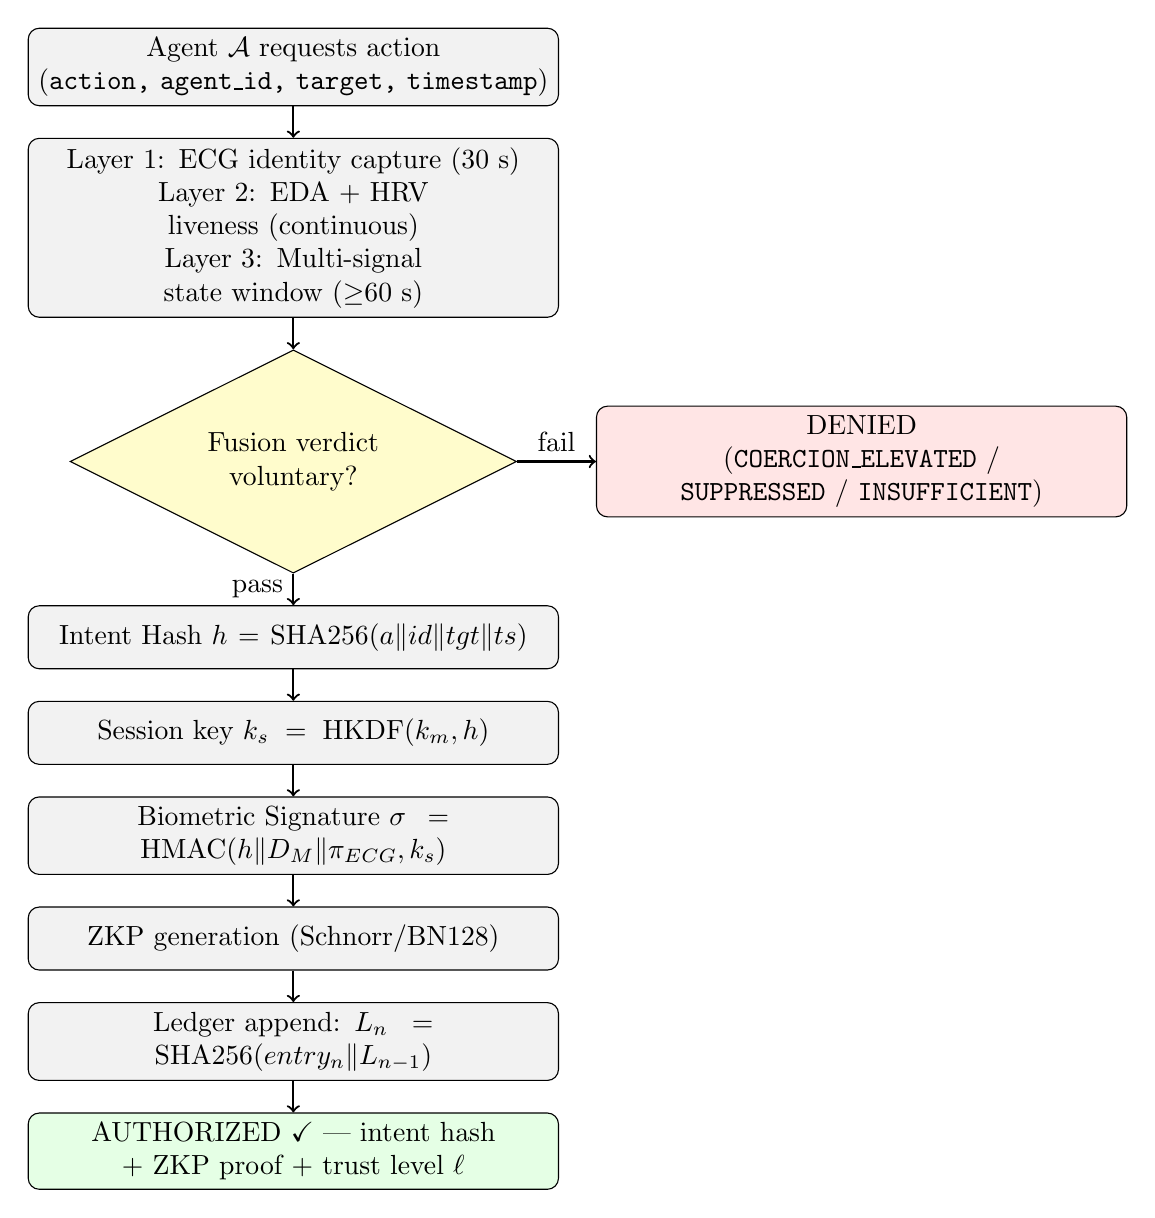
\begin{tikzpicture}[
  box/.style={rectangle, draw, rounded corners, text width=6.5cm,
              align=center, minimum height=0.8cm, fill=gray!10},
  decision/.style={diamond, draw, text width=3.5cm, align=center,
                   fill=yellow!20, aspect=2},
  arrow/.style={->, thick}
]
\node[box] (req)    {Agent $\mathcal{A}$ requests action\\
                     (\texttt{action, agent\_id, target, timestamp})};
\node[box, below=0.4cm of req] (cap)
                    {Layer~1: ECG identity capture (30~s)\\
                     Layer~2: EDA + HRV liveness (continuous)\\
                     Layer~3: Multi-signal state window ($\geq$60~s)};
\node[decision, below=0.4cm of cap] (check)
                    {Fusion verdict\\voluntary?};
\node[box, right=1cm of check, fill=red!10] (deny)
                    {DENIED\\(\texttt{COERCION\_ELEVATED} /
                     \texttt{SUPPRESSED} / \texttt{INSUFFICIENT})};
\node[box, below=0.4cm of check] (hash)
                    {Intent Hash $h = \text{SHA256}(a \| id \| tgt \| ts)$};
\node[box, below=0.4cm of hash] (key)
                    {Session key $k_s = \text{HKDF}(k_m, h)$};
\node[box, below=0.4cm of key] (sig)
                    {Biometric Signature $\sigma = \text{HMAC}(h \| D_M \| \pi_{ECG}, k_s)$};
\node[box, below=0.4cm of sig] (zkp)
                    {ZKP generation (Schnorr/BN128)};
\node[box, below=0.4cm of zkp] (ledger)
                    {Ledger append: $L_n = \text{SHA256}(entry_n \| L_{n-1})$};
\node[box, below=0.4cm of ledger, fill=green!10] (auth)
                    {AUTHORIZED $\checkmark$ — intent hash + ZKP proof + trust level $\ell$};

\draw[arrow] (req) -- (cap);
\draw[arrow] (cap) -- (check);
\draw[arrow] (check) -- node[left]{pass} (hash);
\draw[arrow] (check) -- node[above]{fail} (deny);
\draw[arrow] (hash) -- (key);
\draw[arrow] (key) -- (sig);
\draw[arrow] (sig) -- (zkp);
\draw[arrow] (zkp) -- (ledger);
\draw[arrow] (ledger) -- (auth);
\end{tikzpicture}
\caption{LICET v2 authorization flow with three-layer physiological verification.}
\label{fig:flow}
\end{figure}

\subsection{Three-Layer Physiological Architecture}
\label{sec:threelayer}

LICET v2 replaces single-signal threshold detection with a three-layer
architecture addressing distinct verification properties.

\subsubsection{Layer 1 — Identity Anchor: ECG Waveform Morphology}

ECG waveform morphology (QRS complex shape, PR interval, QT interval, T-wave
morphology) is determined by cardiac anatomy and electrical conduction pathway
geometry. These are individually unique, stable across decades, and
\textbf{impossible to alter pharmacologically} at any clinically relevant dose.

At the start of each authorization session, a 30-second ECG recording is
obtained (Apple Watch Ultra 2 / Series~8+ via \texttt{HKElectrocardiogram} at
512~Hz; Samsung Galaxy Watch~4+ via Samsung Health Monitor). A morphological
match score $\rho_{ECG} \in [0, 1]$ is computed against the enrolled baseline:

\begin{equation}
\rho_{ECG} = \text{cosine\_similarity}\!\left(
  \mathbf{f}(ecg_{\text{session}}),\;
  \mathbf{f}(ecg_{\text{enrolled}})
\right)
\end{equation}

where $\mathbf{f}(\cdot)$ extracts a feature vector of (QRS duration, PR
interval, QTc, axis, T-wave amplitude ratio). Authorization proceeds only if
$\rho_{ECG} \geq \theta_{ECG}$ (default: 0.85).

\subsubsection{Layer 2 — Liveness: EDA and HRV Pattern}

The liveness layer proves that a conscious, awake biological subject is present
and not a replay attack. Two signals contribute:

\textbf{Electrodermal Activity (EDA):} Continuous EDA is available from WHOOP~5
and Fitbit Sense~2. Spot-check EDA ($\geq$3 minutes) is available from Samsung
Galaxy Watch~5/6/7. EDA is controlled by sympathetic cholinergic innervation
and therefore cannot be voluntarily suppressed. A minimum of one skin
conductance response (SCR) with physiologically correct morphology (onset
latency 1--3~s, amplitude $\geq 0.05$~$\mu$S, recovery 5--10~s) must be
present during the session to confirm autonomic reactivity.

\textbf{Overnight HRV Pattern:} The statistical distribution of RMSSD across
sleep stages (not just the mean) carries individual-specific characteristics
that are stable across time but disturbed by pharmacological intervention.
The pattern match score $\rho_{HRV} \in [0, 1]$ is computed against the
enrolled 30-day baseline using distributional distance.

\subsubsection{Layer 3 — Voluntary State: Personalized Mahalanobis Fusion}
\label{sec:fusion}

Layer 3 replaces population-level HR/HRV thresholds with a personalized
multivariate deviation detector over a minimum 60-second capture window.

\textbf{Signal set.} Let $\mathbf{x} = (x_1, \ldots, x_k)$ be the vector of
$k$ physiological features extracted during the authorization window:

\begin{center}
\begin{tabular}{llll}
\toprule
$x_i$ & Signal & Source & Attack resistance \\
\midrule
$x_1$ & RMSSD (ms) & PPG / ECG & Medium (vagal, not beta-blocked) \\
$x_2$ & EDA SCL ($\mu$S) & EDA electrodes & High (cholinergic) \\
$x_3$ & EDA SCR count & EDA electrodes & High \\
$x_4$ & Skin temp delta (°C) & Thermistor & High ($\alpha_1$-adrenergic) \\
$x_5$ & Tremor 8--12~Hz (mg) & IMU $\geq$50~Hz & Inverse (absence = beta-blocker) \\
$x_6$ & Respiratory rate (bpm) & PPG + IMU & High (most attacks) \\
$x_7$ & SpO$_2$ variability (\%) & PPG & Medium \\
\bottomrule
\end{tabular}
\end{center}

\textbf{Personalized z-scores.} For each signal $x_i$, compute the z-score
against the individual's personal baseline $(\mu_i^B, \sigma_i^B)$ estimated
from $\geq 5$ calm sessions of $\geq 3$ minutes each:

\begin{equation}
z_i = \frac{x_i - \mu_i^B}{\sigma_i^B}
\end{equation}

\textbf{Mahalanobis fusion score.} The multivariate deviation from the calm
baseline is:

\begin{equation}
D_M = \sqrt{(\mathbf{z} - \boldsymbol{\mu}_{\text{calm}})^T
\mathbf{S}^{-1}
(\mathbf{z} - \boldsymbol{\mu}_{\text{calm}})}
\label{eq:mahal}
\end{equation}

where $\mathbf{S}$ is the covariance matrix of physiological features during
the individual's calm baseline sessions. $\mathbf{S}$ captures inter-signal
correlations: EDA and HR normally co-elevate under stress; a dissociation
(EDA flat, HR elevated) increases $D_M$ even when each signal appears
individually unremarkable.

\textbf{Verdict mapping:}
\begin{equation}
\text{Verdict}(D_M) =
\begin{cases}
\texttt{CLEAR}     & D_M < \theta_{\text{low}} \\
\texttt{ELEVATED}  & \theta_{\text{low}} \leq D_M < \theta_{\text{high}} \\
\texttt{HIGH}      & D_M \geq \theta_{\text{high}} \\
\texttt{SUPPRESSED}& \text{pharmacological attack pattern detected (Eq.~\ref{eq:pharmattack})}
\end{cases}
\end{equation}

Authorization proceeds only if verdict is \texttt{CLEAR}.

\subsubsection{Pharmacological Attack Pattern Detection}
\label{sec:pharmattack}

A key innovation of LICET v2 is explicit detection of pharmacological
countermeasure patterns. Each attack type produces a characteristic signal
dissociation that the fusion model flags:

\begin{equation}
\text{Attack}(\mathbf{z}) =
\begin{cases}
\texttt{BETA\_BLOCKER}    & z_5 < -2.0
  \;\text{(tremor absent)}
  \land (\Delta HR_{\text{baseline}} > 15\%) \\
\texttt{ANTICHOLINERGIC}  & z_2 < -1.5
  \;\text{(EDA suppressed)}
  \land z_1 > +1.0
  \;\text{(HR elevated)}
  \land x_4 > 0
  \;\text{(skin warm)} \\
\texttt{OPIOID}           & z_6 < -2.0
  \;\text{(respiratory depressed)}
  \land x_4 > 0
  \;\text{(skin warm)}
  \land z_1 < 0
  \;\text{(bradycardia)} \\
\texttt{COMBINED}         & \text{two or more attack patterns simultaneously}
\end{cases}
\label{eq:pharmattack}
\end{equation}

If any attack pattern is detected, the verdict is set to \texttt{SUPPRESSED}
regardless of $D_M$ value. The attack pattern is logged in the ledger.

\textbf{Note on beta-blockers and RMSSD.} A common misconception is that
beta-adrenergic blockers fully suppress HRV. In fact, RMSSD reflects
\emph{parasympathetic} (vagal) withdrawal, not sympathetically mediated
activity \cite{brantigan1982}. Beta-blockers attenuate LF power and raw HR
elevation but do not prevent vagal withdrawal under coercion. Personalized
baseline deviation (not absolute RMSSD value) remains detectable in
beta-blocked individuals. The explicit signal of beta-blockade is tremor
suppression (Eq.~\ref{eq:pharmattack}): physiological tremor at 8--12~Hz is
enhanced by sympathetic beta-adrenergic stimulation and therefore reduced
below baseline by beta-blockers---the \emph{absence} of expected tremor is
the attack detection signal \cite{lakie2019tremor}.

\subsection{Biometric Trust Levels (RATS Alignment)}
\label{sec:trustlevels}

LICET defines four biometric trust levels aligned with IETF RATS
RFC~9334~\cite{rfc9334}, reflecting the attestation capability of the wearable
device:

\begin{description}
  \item[L0 — No Hardware Attestation.] Data originates from cloud API with
  OAuth authentication only (Oura Ring API, Apple HealthKit without App
  Attest, Samsung Health Connect without Knox). Physiological values are
  informative metadata only. Suitable for T1 (software-only) deployments with
  reduced assurance claims.

  \item[L1 — Platform Attestation.] The companion mobile app is attested as
  running on a genuine, unmodified device (Apple DCAppAttest via Secure
  Enclave; Samsung Knox DeviceAttestation). The app's integrity is verified;
  sensor data provenance is not independently verified. Suitable for T2
  (attested software) CPoE tier.

  \item[L2 — Hardware Attestation with Third-Party Verifiable CA.] The device
  holds a hardware-backed attestation key whose certificate chain can be
  verified by any third party without contacting the manufacturer's server.
  Currently achievable with Google Pixel Watch~2 + Android Key Attestation
  (Titan~M2 security chip; Google publishes the hardware attestation root CA).
  Suitable for T3 (hardware-bound) with explicit caveats on sensor data path.

  \item[L3 — Sensor-to-TEE Direct Attestation (Future Standard).] The
  wearable MCU signs sensor data \emph{inside the trusted execution
  environment before the application processor can observe it}. The signing
  key is provisioned at manufacturing time and included in an Endorser
  certificate chain. No commercially available consumer wearable implements
  this architecture as of 2026. LICET defines this level as the target
  specification for future wearable hardware, providing a clear standard
  against which manufacturers can certify compliance. Suitable for T4
  (hardware-hardened) deployments with the highest forgery-cost guarantees.
\end{description}

The biometric trust level $\ell$ is reported in the ledger entry and the ZKP
proof, allowing Relying Parties to make risk-appropriate trust decisions per
RFC~9334 Section~3.

\textbf{Composite Attester Topology (RFC~9334 §3.1.4).} In LICET's RATS
role mapping, the wearable device acts as a \emph{Sub-Attester} producing
physiological Evidence (signed at levels L1--L3 by the device's attestation
key). The smartphone acts as \emph{Lead Attester}, aggregating Sub-Attester
Evidence with platform-level Evidence before presenting the composite Evidence
packet to the LICET Verifier. This topology is architecturally valid under
RFC~9334 but requires formal specification of the Sub-Attester Evidence format
and Endorser trust chain---an open standardization gap that LICET addresses
through its L3 specification target.

\subsection{Baseline Capture Protocol}
\label{sec:baseline}

The personalized baseline is a prerequisite for Layers 2 and 3.

\begin{itemize}
  \item \textbf{Initial enrollment:} $\geq 5$ sessions of $\geq 3$ minutes
  each in a verified calm state, capturing ECG (Layer~1 enrollment), EDA SCL
  distribution, and all Layer~3 signals.
  \item \textbf{Minimum time to first authorization:} 24 hours after last
  baseline session.
  \item \textbf{Baseline expiry:} 30 days. Re-enrollment required after
  expiry.
  \item \textbf{Baseline anomaly detection:} If resting HR deviates $>15\%$
  from historical resting baseline, or EDA SCL is $<50\%$ of historical
  baseline, the baseline session is flagged and excluded. This detects
  pre-authorization beta-blocker or anticholinergic pre-medication.
\end{itemize}

The baseline digest $H_B = \text{HMAC}(\mu_B \| \Sigma_B \| t_B, k_m)$ is
stored server-side and referenced in each authorization ledger entry.

\subsection{Intent Hash}
\label{sec:intent-hash}

The Intent Hash uniquely and immutably identifies the requested action:

\begin{equation}
h = \text{SHA256}(a \,\|\, id_{\mathcal{A}} \,\|\, tgt \,\|\, ts \,\|\, \ell)
\end{equation}

where $a$ is the action descriptor, $id_{\mathcal{A}}$ the agent identifier,
$tgt$ the target entity, $ts$ a Unix timestamp, and $\ell$ the biometric
trust level. Any single-bit modification to any field produces a completely
different $h$.

\subsection{Session Key Derivation}

A per-event session key is derived using HKDF \cite{krawczyk2010hkdf}:

\begin{equation}
k_s = \text{HKDF-SHA256}(k_m,\, h)
\end{equation}

where $k_m$ is the server master key. This ensures that compromise of one
session key does not affect any other authorization event.

\subsection{Biometric Signature}

The Biometric Temporal Signature commits the physiological state to the intent
hash:

\begin{equation}
\sigma = \text{HMAC-SHA256}\!\left(
  h \,\|\, D_M \,\|\, \rho_{ECG} \,\|\, \text{verdict} \,\|\, \ell \,\|\, ts,\;
  k_s\right)
\end{equation}

Properties:
\begin{itemize}
  \item \textbf{Event-unique:} $ts$ ensures no replay across distinct events.
  \item \textbf{Action-bound:} $h$ is embedded; $\sigma$ cannot be transferred
  to authorize a different action.
  \item \textbf{Non-invertible:} no biometric value can be recovered from
  $\sigma$ without $k_s$.
  \item \textbf{Fusion-committed:} $D_M$ commits the full multivariate fusion
  result without exposing individual signal values.
\end{itemize}

\subsection{Zero-Knowledge Proof}
\label{sec:zkp}

LICET uses a non-interactive Schnorr proof over BN128 with the Fiat-Shamir
transform \cite{fiat1987}. This allows any auditor $\mathcal{V}$ to verify
that a valid multi-modal biometric authorization exists without learning any
physiological values.

\textbf{Setup.} Let $\mathbb{G}$ be the BN128 group of prime order $q$, with
generator $G$.

\textbf{Proof generation by $\mathcal{S}$:}
\begin{align}
w   &= \text{SHA256}(\sigma \,\|\, h) \bmod q \\
PK  &= w \cdot G \\
r   &\stackrel{\$}{\leftarrow} \mathbb{Z}_q \\
R   &= r \cdot G \\
c   &= \text{SHA256}(R \,\|\, PK \,\|\, h) \bmod q \\
s   &= (r - c \cdot w) \bmod q
\end{align}

The proof $\pi = (R, c, s, PK)$ is stored in the ledger alongside the
authorization record.

\textbf{Verification by $\mathcal{V}$:}
\begin{equation}
s \cdot G + c \cdot PK \stackrel{?}{=} R
\label{eq:verify}
\end{equation}

If Equation~\ref{eq:verify} holds and $c = \text{SHA256}(R \,\|\, PK \,\|\,
h) \bmod q$, the auditor is convinced that a valid multi-modal biometric
authorization exists, without learning $D_M$, $\rho_{ECG}$, or any
individual signal value.

\subsection{Hash-Chained Ledger}

Every authorization event is appended to a hash-chained ledger:

\begin{align}
L_0 &= \text{SHA256}(entry_0 \,\|\, \texttt{"GENESIS"}) \\
L_n &= \text{SHA256}(entry_n \,\|\, L_{n-1}), \quad n \geq 1
\end{align}

where $entry_n$ contains the intent hash, fusion verdict, pharmacological
attack flags (if any), trust level $\ell$, ZKP proof $\pi$, and timestamp.
The ledger endpoint \texttt{GET /v1/ledger/integrity} recomputes the full
chain, allowing any observer to detect retroactive tampering without a trusted
third party.

% ──────────────────────────────────────────────────────────────────────────────
\section{Security Analysis}
% ──────────────────────────────────────────────────────────────────────────────

\subsection{Threat Model}

We consider the following adversarial capabilities:
\begin{enumerate}
  \item \textbf{Credential compromise:} adversary obtains passwords, biometric
  templates, or private keys.
  \item \textbf{Replay attack:} adversary captures a valid LICET token and
  replays it for a different action or at a later time.
  \item \textbf{Physical coercion:} adversary physically threatens the
  authorizer.
  \item \textbf{Cognitive incapacitation:} the authorizer is sedated, hypoxic,
  or unconscious.
  \item \textbf{Beta-adrenergic blockade:} adversary pre-medicates the
  authorizer with propranolol or metoprolol to suppress sympathetic responses.
  \item \textbf{Anticholinergic suppression:} adversary administers atropine,
  scopolamine, or glycopyrrolate to suppress EDA.
  \item \textbf{Opioid sedation:} adversary administers opioids to impair
  respiratory and autonomic responses.
  \item \textbf{Combined pharmacological attack:} adversary combines multiple
  agents to suppress all channels simultaneously.
  \item \textbf{Ledger tampering:} adversary retroactively alters authorization
  records.
  \item \textbf{Privacy attack:} a curious auditor attempts to extract
  biometric data from the authorization record.
  \item \textbf{Key compromise:} the server master key $k_m$ is exposed.
\end{enumerate}

\subsection{Security Properties}

\begin{description}
  \item[P1 — Credential independence.] Even with all credentials, an adversary
  who cannot produce valid real-time multi-modal physiological state cannot
  obtain a valid LICET token.

  \item[P2 — Replay resistance.] The session key $k_s = \text{HKDF}(k_m, h)$
  is unique per intent hash $h$, which includes action, target, timestamp, and
  trust level.

  \item[P3 — Coercion cost elevation.] The three-layer architecture raises the
  cost of obtaining unauthorized authorization under coercion. No known
  single-agent pharmacological attack defeats all layers simultaneously at
  survivable doses.

  \item[P4 — Beta-blocker resistance.] Tremor suppression detection (Layer~3,
  $z_5 < -2.0$) and personal baseline shift detection in baseline sessions
  detect beta-adrenergic pre-medication. RMSSD vagal withdrawal persists under
  beta-blockade and remains detectable via personalized z-scoring.

  \item[P5 — Anticholinergic resistance.] EDA suppression combined with HR
  elevation and warm skin temperature (inverted stress pattern) detects
  anticholinergic administration. The toxidrome (tachycardia, dry flushed
  skin, possible confusion) creates a recognizable signal dissociation.

  \item[P6 — Identity anchor pharmacological resistance.] ECG morphology
  (Layer~1) cannot be altered by any medication. An authorized person's QRS
  complex, PR interval, and QT interval remain their personal anatomical
  signature regardless of pharmacological intervention.

  \item[P7 — Combined attack self-defeat.] The drug combination required to
  suppress all channels simultaneously (beta-blocker + anticholinergic +
  alpha-blocker) produces severe hemodynamic instability (hypotension,
  tachycardia, reflex bradycardia collision) that would incapacitate the
  subject before physiological normalization is achieved across all channels.

  \item[P8 — Ledger integrity.] Any modification to ledger entry $L_i$
  invalidates $L_{i+1}, \ldots, L_n$, making tampering mathematically
  detectable.

  \item[P9 — Biometric privacy.] The ZKP provides zero-knowledge: auditors
  learn that a valid multi-modal authorization exists but gain no information
  about $D_M$, $\rho_{ECG}$, or any individual signal value.

  \item[P10 — Session key isolation.] HKDF derivation ensures compromise of
  session key $k_s^{(i)}$ does not expose $k_s^{(j)}$ or $k_m$.
\end{description}

\subsection{Estimated Error Rates}

Based on the WESAD benchmark \cite{schmidt2018wesad} and follow-on multi-signal
fusion literature \cite{healey2005stress, gjoreski2017stress}:

\begin{itemize}
  \item 2-signal fusion (EDA + HRV, population model): FNR $\approx 8\%$, FPR
  $\approx 10\%$.
  \item 4-signal fusion with personalized baseline: FNR $\approx 2\%$, FPR
  $\approx 4\%$.
  \item 5-signal fusion + pharmacological attack detection + personalized
  baseline: estimated FNR $1\text{--}2\%$, FPR $3\text{--}5\%$.
\end{itemize}

These estimates are for laboratory-grade sensor hardware. Consumer PPG-based
HRV has higher variance than research-grade sensors; clinical deployments
should require ECG-quality HR for Layer~1 and EDA-capable devices for
full Layer~2 and Layer~3 guarantees.

\subsection{Acknowledged Limitations}

\begin{enumerate}
  \item \textbf{EDA hardware availability.} Continuous EDA is available on
  WHOOP~5 and Empatica EmbracePlus; spot-check EDA on Samsung Galaxy Watch~5+
  and Fitbit Sense~2. Apple Watch, Oura Ring, and Garmin devices do not expose
  EDA as of 2026. Deployments on non-EDA devices operate at reduced liveness
  assurance.

  \item \textbf{L3 not yet commercially available.} No consumer wearable as of
  2026 provides direct sensor-to-TEE attestation. L2 (Pixel Watch~2 + Android
  Key Attestation) is the highest hardware assurance achievable today.

  \item \textbf{Baseline cold start.} Five sessions are required before first
  authorization. Users cannot use LICET immediately upon enrollment.

  \item \textbf{Anticholinergic detection requires EDA.} Without an EDA
  sensor, anticholinergic attacks are harder to detect. The warm-skin +
  HR-elevated pattern in temperature and HRV provides partial detection.

  \item \textbf{Server trust.} The current architecture trusts the LICET
  server. Decentralized execution (smart-contract ZKP verifier) is a future
  direction.
\end{enumerate}

% ──────────────────────────────────────────────────────────────────────────────
\section{Implementation}
% ──────────────────────────────────────────────────────────────────────────────

\subsection{Server}

The reference implementation is a Python/FastAPI application deployed on Google
Cloud Run (\texttt{us-central1}). The cryptographic stack uses:

\begin{itemize}
  \item \texttt{cryptography} (Python): HKDF-SHA256, HMAC-SHA256
  \item \texttt{py\_ecc}: Schnorr proof over BN128
  \item \texttt{SQLite}: hash-chained ledger persistence
  \item \texttt{numpy/scipy}: Mahalanobis distance computation, baseline
  covariance estimation
\end{itemize}

The API is publicly accessible at \texttt{https://licet.dev/v1/}.

\subsection{Android Application}

A companion Android application (Kotlin, Jetpack Compose) integrates with
Samsung Health Connect to read HR, HRV, EDA (Galaxy Watch~5+), skin
temperature, and accelerometer data. The app implements the full LICET
onboarding flow including baseline capture, real-time authorization UI, and
trust level reporting.

\subsection{Supported Wearable Platforms}

\begin{center}
\begin{tabular}{lllll}
\toprule
\textbf{Device} & \textbf{ECG} & \textbf{EDA} & \textbf{Trust Level} & \textbf{Tier} \\
\midrule
Apple Watch Ultra~2 / S9+ & \checkmark (512~Hz) & \texttimes & L1 & T2 \\
Samsung Galaxy Watch~7 & \checkmark (512~Hz) & Spot-check & L1 & T2 \\
Google Pixel Watch~2 & \texttimes & \texttimes & L2 & T3 \\
WHOOP~5 & \texttimes & \checkmark (continuous) & L0 & T1 \\
Oura Ring~4/5 & \texttimes & \texttimes & L0 & T1 \\
Apple Watch + WHOOP~5 & \checkmark & \checkmark & L1 & T2 \\
Pixel Watch~2 + WHOOP~5 & \texttimes & \checkmark & L2 & T3 \\
\bottomrule
\end{tabular}
\end{center}

\subsection{REST API}

\begin{center}
\begin{tabular}{llp{6.5cm}}
\toprule
\textbf{Method} & \textbf{Endpoint} & \textbf{Description} \\
\midrule
GET  & \texttt{/v1/health}              & Protocol liveness check \\
POST & \texttt{/v1/authorize}           & Full multi-modal authorization \\
POST & \texttt{/v1/biometric/push}      & Wearable push (app $\to$ server) \\
POST & \texttt{/v1/authorize/from-push} & Authorize using pushed biometrics \\
POST & \texttt{/v1/verify}             & ZKP verification (auditors) \\
GET  & \texttt{/v1/ledger/integrity}    & Full chain integrity check \\
GET  & \texttt{/v1/ledger/history}      & Authorization event history \\
\bottomrule
\end{tabular}
\end{center}

\subsection{Minimal Integration Example}

\begin{lstlisting}[language=Python, caption={Minimal LICET v2 authorization request.}]
import requests

response = requests.post("https://licet.dev/v1/authorize", json={
    "action":            "prescribe_insulin_50ui",
    "agent_id":          "medical_agent_v1",
    "target":            "patient_id_12345",
    "window_seconds":    60,       # minimum 60s capture window
    "trust_level":       1,        # L1: App Attest device binding
    "ecg_features":      {...},    # QRS/PR/QT from Apple Watch
    "eda_scl":           4.2,      # microsiemens
    "eda_scr_count":     3,
    "hrv_rmssd":         42.1,     # ms
    "skin_temp_delta":   -0.8,     # degrees C (negative = vasoconstriction)
    "tremor_8_12hz":     3.2,      # mg RMS
    "respiratory_rate":  15.4      # breaths/min
}, headers={"X-LICET-App-Secret": "<app_secret>"})

result = response.json()
if result["authorized"]:
    intent_hash = result["intent_hash"]
    zkp_proof   = result["zkp_proof"]
    trust_level = result["trust_level"]     # L0-L3
    fusion_dm   = result["mahalanobis_distance"]
else:
    verdict     = result["verdict"]         # ELEVATED / HIGH / SUPPRESSED
    attack_flag = result.get("attack_pattern")  # BETA_BLOCKER / ANTICHOLINERGIC / etc.
\end{lstlisting}

% ──────────────────────────────────────────────────────────────────────────────
\section{Use Cases}
% ──────────────────────────────────────────────────────────────────────────────

\textbf{Healthcare.} AI agents prescribing controlled medications or adjusting
treatment protocols require oversight that is verifiably free from duress. The
ECG identity anchor confirms the correct physician; the EDA liveness layer
confirms conscious presence; the Mahalanobis fusion confirms voluntary state.

\textbf{Finance.} High-value autonomous transactions require authorization
demonstrably free from coercion or pharmacological manipulation. LICET's
pharmacological attack pattern detection and ledger provide a legally auditable
trail.

\textbf{Critical infrastructure.} Operations modifying power grids,
telecommunications, or water systems via AI agents demand oversight that is
both real and verifiable. LICET's ZKP layer allows independent auditors to
verify human oversight without accessing operational biometrics.

\textbf{Legal and compliance.} Regulated AI decisions require documented human
supervision. LICET's machine-verifiable, privacy-preserving audit record is
compatible with e-signature and records-management frameworks.

% ──────────────────────────────────────────────────────────────────────────────
\section{Regulatory Alignment}
% ──────────────────────────────────────────────────────────────────────────────

\textbf{EU AI Act (Regulation 2024/1689).}
LICET addresses operational human oversight obligations under three distinct
provisions:

\textit{Article~9 (Risk Management System)} requires providers to implement
ongoing monitoring of high-risk AI systems including documented human oversight
events. LICET's hash-chained ledger provides the tamper-evident record of each
oversight event with physiological state attestation.

\textit{Article~12 (Record-Keeping)} mandates automatic logging of events
enabling post-hoc reconstruction of AI system behavior and oversight actions.
LICET's ledger satisfies this requirement with ZKP-protected entries that
preserve biometric privacy.

\textit{Article~26(5) (Deployer Obligations)} requires deployers of high-risk
AI systems to ensure human oversight is genuinely exercised. LICET provides
the evidentiary layer that distinguishes genuine (voluntary, conscious,
uncoerced) from nominal (button-pressed-under-duress) oversight.

Note: Article~14 governs the AI system's \emph{design capacity} for human
oversight---requiring that the system architecture permit monitoring and
intervention. LICET addresses the complementary \emph{operational assurance}
question of whether that capacity was genuinely exercised in a specific
instance, as required by Articles~9, 12, and 26.

\textbf{CEN-CENELEC JTC~21 (EU AI Act Harmonised Standards).} The ongoing
harmonised standards process under the EU AI Act will define what conformity
assessments require for demonstrating genuine human oversight. LICET's
physiological attestation approach is directly relevant to these standards as
they develop.

\textbf{Brazil LGPD (Lei 13.709/2018).} LICET's ZKP design ensures that
biometric data (LGPD Article~5, sensitive personal data) is never stored in
the ledger or exposed to auditors. The authorization proof is functionally
separated from the physiological values that generated it.

\textbf{NIST AI Risk Management Framework.} The GOVERN and MEASURE functions
call for documentation of human oversight events. LICET's hash-chained ledger
provides tamper-evident records of each oversight event.

% ──────────────────────────────────────────────────────────────────────────────
\section{Open Research Problems}
% ──────────────────────────────────────────────────────────────────────────────

\begin{enumerate}
  \item \textbf{Level~3 (Sensor-to-TEE) specification and standardization.}
  No consumer wearable currently provides direct sensor-to-TEE attestation.
  This paper defines the L3 architecture target; IEEE and IETF standardization
  of the hardware profile is an open research and standardization problem with
  significant security implications.

  \item \textbf{Composite Attester profile for RFC~9334.} Formally specifying
  the wearable as a Sub-Attester in the RATS Composite Device model requires:
  (a) Sub-Attester Evidence format in CBOR/EAT; (b) Lead Attester aggregation
  obligations; (c) Endorser trust chain for wearable manufacturer certificates;
  (d) Verifier appraisal policy for composite physiological Evidence. This is
  an open IETF contribution opportunity.

  \item \textbf{Clinical validation of pharmacological attack detection.}
  Prospective studies measuring specificity and sensitivity of the attack
  pattern detection in Equation~\ref{eq:pharmattack} against controlled
  pharmacological administration are needed to validate the detection thresholds.

  \item \textbf{Baseline poisoning attacks.} An adversary who can control the
  baseline capture environment (e.g., administering medication during baseline
  sessions) may shift the personal baseline to accommodate coerced states.
  Anomaly detection for baseline sessions (Section~\ref{sec:baseline}) provides
  partial mitigation; formal analysis of baseline poisoning bounds is needed.

  \item \textbf{Decentralized verifier.} Deploying the ZKP verifier as an
  EVM-compatible smart contract eliminates server trust assumptions. The
  Mahalanobis computation and pharmacological pattern detection could be
  implemented as on-chain Groth16 proofs.

  \item \textbf{Multi-modal liveness hardening.} Combining physiological
  signals with NFC document verification, facial liveness detection, and
  behavioral biometrics for higher assurance levels, particularly for
  deployments without EDA-capable hardware.

  \item \textbf{Formal protocol verification.} Mechanized proof of LICET's
  security properties using ProVerif or Tamarin, particularly the
  pharmacological attack detection guarantees.

  \item \textbf{Threshold standardization.} Collaboration with regulatory
  bodies to define minimum required biometric trust levels (L0--L3) and fusion
  thresholds for different risk categories of AI agent actions.
\end{enumerate}

% ──────────────────────────────────────────────────────────────────────────────
\section{Conclusion}
% ──────────────────────────────────────────────────────────────────────────────

We have presented LICET v2, a cryptographic middleware protocol that closes the
intent gap in AI agent authorization through a three-layer physiological
architecture. By anchoring identity in pharmacologically invariant ECG
morphology, confirming liveness through electrodermal activity that cannot be
voluntarily suppressed, detecting pharmacological attack patterns through
signal dissociation analysis, and fusing all signals via personalized
Mahalanobis distance, LICET provides meaningful resistance to the full space
of known countermeasures---credential theft, physical coercion, and
pharmacological manipulation.

The four-level biometric trust hierarchy (L0--L3), formally aligned with IETF
RATS RFC~9334, provides a progression path from today's software-only
deployments to future sensor-to-TEE hardware, defining the standard that
wearable manufacturers should implement. The ZKP layer ensures that this
comprehensive physiological verification leaves no biometric trace accessible
to auditors.

The protocol is implemented and publicly deployed. The open research problems
above---particularly the L3 hardware specification and RATS Composite Attester
profile---represent an invitation to the IETF, IEEE, and wearable hardware
communities to build the infrastructure that makes this protocol's highest
assurance level achievable at scale.

\textit{LICET---``it is permitted''---because conscious, free, and
physiologically verified human intent must be the irreducible foundation of
any AI action with real consequences.}

% ──────────────────────────────────────────────────────────────────────────────
\section*{Availability}
% ──────────────────────────────────────────────────────────────────────────────

Reference implementation: \href{https://licet.dev}{\texttt{https://licet.dev}}\\
IETF Internet-Draft: \href{https://datatracker.ietf.org/doc/draft-pereira-licet-human-intent/}{\texttt{draft-pereira-licet-human-intent-01}}\\
SSRN Preprint: \href{https://papers.ssrn.com/sol3/papers.cfm?abstract_id=7018458}{\texttt{Abstract ID 7018458}}\\
Blockchain timestamp: eColabs\_LICET\_Protocol\_v1.pdf.ots (OpenTimestamps / Bitcoin, 2026-02-25)

% ──────────────────────────────────────────────────────────────────────────────
\section*{Conflict of Interest}
% ──────────────────────────────────────────────────────────────────────────────

The author is the sole founder of eColabs Desenvolvimento de Pessoas e
Organizações LTDA.\ and creator of the LICET protocol.

% ──────────────────────────────────────────────────────────────────────────────
\begin{thebibliography}{99}

\bibitem{euaiact2024}
European Parliament and of the Council.
\textit{Regulation (EU) 2024/1689 of the European Parliament and of the
Council laying down harmonised rules on artificial intelligence (Artificial
Intelligence Act)}, June 2024.

\bibitem{nistairimf2023}
National Institute of Standards and Technology.
\textit{Artificial Intelligence Risk Management Framework (AI RMF 1.0)}.
NIST AI 100-1, January 2023.

\bibitem{rfc9334}
H.~Birkholz, D.~Thaler, M.~Richardson, N.~Smith, and W.~Pan.
\textit{Remote ATtestation procedureS (RATS) Architecture}.
RFC 9334, Internet Engineering Task Force, January 2023.

\bibitem{thayer2012hrv}
J.~F. Thayer, F.~\AA{}hs, M.~Fredrikson, J.~J. Sollers~III, and T.~D. Wager.
A meta-analysis of heart rate variability and neuroimaging studies: Implications
for heart rate variability as a marker of stress and health.
\textit{Neuroscience \& Biobehavioral Reviews}, 36(2):747--756, 2012.

\bibitem{kim2018stress}
H.-G. Kim, E.-J. Cheon, D.-S. Bai, Y.~H. Lee, and B.-H. Koo.
Stress and heart rate variability: A meta-analysis and review of the literature.
\textit{Psychiatry Investigation}, 15(3):235--245, 2018.

\bibitem{selye1956stress}
H.~Selye.
\textit{The Stress of Life}.
McGraw-Hill, New York, 1956.

\bibitem{schmidt2018wesad}
P.~Schmidt, A.~Reiss, R.~Duerichen, C.~Marberger, and K.~Van Laerhoven.
{WESAD}: A multimodal dataset for wearable stress and affect detection.
In \textit{Proceedings of the 20th ACM International Conference on Multimodal
Interaction (ICMI 2018)}, pp.~400--408. ACM, 2018.

\bibitem{healey2005stress}
J.~A. Healey and R.~W. Picard.
Detecting stress during real-world driving tasks using physiological sensors.
\textit{IEEE Transactions on Intelligent Transportation Systems},
6(2):156--166, 2005.

\bibitem{gjoreski2017stress}
M.~Gjoreski, H.~Gjoreski, M.~Lustrek, and M.~Gams.
Monitoring stress with a wrist device using context.
\textit{Journal of Biomedical Informatics}, 73:159--170, 2017.

\bibitem{fowles1986eda}
D.~C. Fowles.
The eccrine system and electrodermal activity.
In M.~G.~H. Coles, E.~Donchin, and S.~W. Porges (Eds.),
\textit{Psychophysiology: Systems, Processes, and Applications},
pp.~51--96. Guilford Press, New York, 1986.

\bibitem{venables1980eda}
P.~H. Venables and M.~J. Christie.
Electrodermal activity.
In I.~Martin and P.~H. Venables (Eds.),
\textit{Techniques in Psychophysiology}, pp.~3--67. Wiley, Chichester, 1980.

\bibitem{brantigan1982}
C.~O. Brantigan, T.~A. Brantigan, and N.~Joseph.
Effect of beta blockade and beta stimulation on stage fright.
\textit{The American Journal of Medicine}, 72(1):88--94, 1982.

\bibitem{lakie2019tremor}
M.~Lakie and C.~A. Vernooij.
The origins of physiological tremor and the role of the muscle spindle.
\textit{The Journal of Physiology}, 597(17):4491--4504, 2019.

\bibitem{israel2005ecg}
S.~A. Israel, J.~M. Irvine, A.~Cheng, M.~D. Wiederhold, and B.~K. Wiederhold.
ECG to identify individuals.
\textit{Pattern Recognition}, 38(1):133--142, 2005.

\bibitem{shaffer2017hrv}
F.~Shaffer and J.~P. Ginsberg.
An overview of heart rate variability metrics and norms.
\textit{Frontiers in Public Health}, 5:258, 2017.

\bibitem{braithwaite2013eda}
J.~J. Braithwaite, D.~G. Watson, R.~Jones, and M.~Rowe.
A guide for analysing electrodermal activity (EDA) \& skin conductance
responses (SCRs) for psychological experiments.
\textit{Psychophysiology}, 2013.

\bibitem{fiat1987}
A.~Fiat and A.~Shamir.
How to prove yourself: Practical solutions to identification and signature
problems.
In \textit{Advances in Cryptology --- CRYPTO '86}, Lecture Notes in Computer
Science, vol.~263, pp.~186--194. Springer, 1987.

\bibitem{krawczyk2010hkdf}
H.~Krawczyk and P.~Eronen.
\textit{HMAC-based Extract-and-Expand Key Derivation Function (HKDF)}.
RFC 5869, Internet Engineering Task Force, May 2010.

\bibitem{camenisch1997}
J.~Camenisch and M.~Stadler.
Efficient group signature schemes for large groups.
In \textit{Advances in Cryptology --- CRYPTO '97}, Lecture Notes in Computer
Science, vol.~1294, pp.~410--424. Springer, 1997.

\bibitem{sasson2014zerocash}
E.~B. Sasson, A.~Chiesa, C.~Garman, M.~Green, I.~Miers, E.~Tromer, and
M.~Virza.
Zerocash: Decentralized anonymous payments from Bitcoin.
In \textit{2014 IEEE Symposium on Security and Privacy}, pp.~459--474, 2014.

\bibitem{laurie2014}
B.~Laurie, A.~Langley, and E.~Kasper.
\textit{Certificate Transparency}.
RFC 6962, Internet Engineering Task Force, June 2013.

\bibitem{schneier1998secure}
B.~Schneier and J.~Kelsey.
Secure audit logs to support computer forensics.
\textit{ACM Transactions on Information and System Security},
2(2):159--176, 1999.

\bibitem{niinuma2010continuous}
K.~Niinuma, U.~Park, and A.~K. Jain.
Soft biometric traits for continuous user authentication.
\textit{IEEE Transactions on Information Forensics and Security},
5(4):771--780, 2010.

\bibitem{Traore2012ImplicitAU}
I.~Traore and A.~A.~E. Ahmed.
\textit{Continuous Authentication Using Biometrics: Data, Models, and Metrics}.
IGI Global, 2012.

\bibitem{Capkun2006}
S.~Capkun, M.~Cagalj, and M.~Srivastava.
Secure localization with hidden and mobile base stations.
In \textit{Proceedings of IEEE INFOCOM}, 2006.

\bibitem{hdp2026}
A.~Dalugoda.
HDP: A Lightweight Cryptographic Protocol for Human Delegation Provenance
in Agentic AI Systems.
Preprint, Helixar Limited, Auckland, New Zealand, March 2026.
IETF Internet-Draft: draft-helixar-hdp-agentic-delegation-00.
\href{https://arxiv.org/abs/2604.04522}{\texttt{arXiv:2604.04522}}.

\bibitem{zerosentinel2026}
ZeroBiometrics.
ZeroSentinel: Cryptographic Human Authorization for Agentic AI Systems.
Technical white paper, March 2026.

\bibitem{beforetoolcall2026}
Anonymous.
Before the Tool Call: Deterministic Pre-Action Authorization for Autonomous
AI Agents.
arXiv preprint arXiv:2603.20953, March 2026.

\end{thebibliography}

\end{document}
